\documentclass[a4paper,fleqn,usenatbib]{mnras}

\usepackage{graphicx}	% Including figure files
\usepackage{amsmath}	% Advanced maths commands
\usepackage{amssymb}	% Extra maths symbols

\title[Human and machine classifications]{A transient search using combined human and machine classifications}

\author[D. Wright, C. Lintott, K. Smith et al.]{
Darryl Wright,$^{1}$\thanks{E-mail: daryll@zooniverse.org}
Chris Lintott,$^{1}$
Ken Smith,$^{2}$
\\
$^{1}$Department of Physics, University of Oxford, Denys Wilkinson Building, Keble Road, Oxford, OX1 3RH
$^{2}$QUBs
}

\date{Accepted XXX. Received YYY; in original form ZZZ}

\pubyear{2016}

\begin{document}
\label{firstpage}
\pagerange{\pageref{firstpage}--\pageref{lastpage}}
\maketitle

% Abstract of the paper
\begin{abstract}
Large modern surveys require efficient review of data in order to find transient sources such as supernovae, and to distinguish such sources from artefacts, noise and so on. Much effort has been put into the development of automatic algorithms, but surveys still rely on human review of targets. This paper presents an integrated system for the identification of supernovae in data from PanSTARRS, combining classifications from a citizen science project including volunteers with those from a convolutional neural network. This work represents the first time such a system has been deployed on real astronomical data, and we show that the combination of the two methods outperforms either one used individually. This result has important implications for the future development of transit searches, especially in the era of LSST and other large-throughput surveys. 
\end{abstract}

\begin{keywords}
keyword1 -- keyword2 -- keyword3
\end{keywords}

%%%%%%%%%%%%%%%%%%%%%%%%%%%%%%%%%%%%%%%%%%%%%%%%%%

%%%%%%%%%%%%%%%%% BODY OF PAPER %%%%%%%%%%%%%%%%%%

\section{Introduction}

\textbf{CJL}

The detection and identification of transient sources has long been an important part of astronomical observation. New surveys such as LSST (XXXXXX CITE XXXXX) will increase the number of transient candidates detected by many orders of magnitude, leading to renewed attention being paid to the methods used by transit searches. 




\section{Method}
\subsection{Pan-STARRS}
\ref{sec:ps1}
Presumably can be grabbed from elsewhere - \textbf{DW}

Using data from MJD57570 and MJD 57586 for the original experiemnt, then 

\subsection{Convolutional Neural Network}

\textbf{DW}

Explain how this was trained (9000 hand-labelled) 
\subsection{Citizen Science Platform}

\textbf{CL}

XXXXX How many people and speed ? Screenshot XXXX \text{DW}
Supernova Hunters began with a beta test on 13th June 2016 and launched on the 12th July 2016 (MJD 57581).  As of the 3rd September 2016 the project has accumulated 426481 classifications from 3158 citizen scientists.  So far citizen scientists have classified 52291 individual subjects corresponding to TTI observations (see Section~\ref{sec:ps1}) of 18838 PS1 objects.  Every Tuesday $\sim5200$ new subjects are uploaded to the project consisting of the previous week's detections that pass our machine cuts.  We require at least 7 citizen scientist classifications before a subject is considered classified and each week's data takes about two days to fully classify.  High confidence (typically $P(real)>0.8$) supernova candidates are screened by experts to remove a small number of false positives before the targets are submitted to the Transient Name Server (TNS).  To date citizen scientists have discovered two hundred supernova candidates submitted to the TNS and two confirmed Supernovae including SN 2016els; a superluminous supernova Type I [XXXXX cite Gal-Yam?? XXXXX].  The classification spectra were obtained by PESSTO [XXXXX cite Smartt XXXXX].
\section{Performance}

The machine is used to identify a cutoff above which candidates are presented to human classifiers; this cutoff is chosen so that a 5\% false positive rate is acheived. This threshold involves a missed detection rate of 5.2\%. We present the results of this machine classification in figure \ref{fig:machine_dist}. A major contaminant is the presence of asteroids; they appear in the dataset as supernovae but are identified here via cross-matching with the Minor Planet Centre ephemaris database (XXXXXX). 

These data were additionally reviewed by at least one expert members of the team (normally DW or KS) to identify genuine supernovae. Candidates were divided into `real' and `bogus' categories based on these expert classifications. 

\begin{figure}
   %\vspace{200pt}
   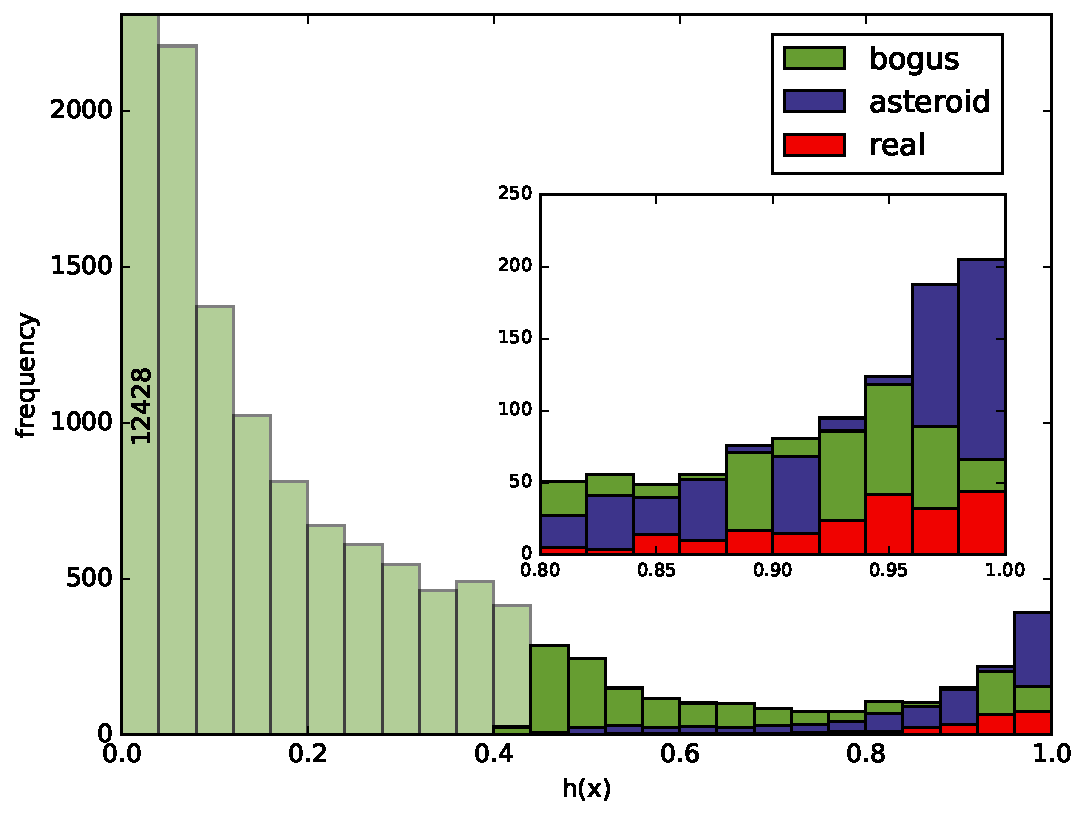
\includegraphics[width=84mm]{figs/machine_hist.pdf}
   \caption{The distribution of $P(real)$ from the current 3$\pi$ machine classifier 
            for detected objects between MJD 57570 and MJD 57586.  The light green shows the distribution of 
            objects with $P(real) < 0.436$ which are automatically rejected.  The remaining 
            objects promoted for human screening even at high values of $P(real)$ contains
            many false positives.} 
   \label{fig:machine_dist} 
\end{figure}

Candidates with high probability as assigned by the machine are more likely to be real. However, although the machine successfully rejects the majority of bogus candidates, the sample produced by the simple cut on probability is far from pure; 1403 real candidates from 3384 in the sample. Higher cutoffs run the risk of rejecting an increasing number of real candidates; requiring a 1\% false positive rate will result in a missed detection rate of 60.3\%. 

An obvious solution to this problem is to improve the performance of the neural network, which, very broadly, is a function of the size of training set. Increasing the training set both directly improves performance but also allows for deeper, more complex networks to be built. However, it is obvious already that obtaining large, clean training sets is expensive, requiring the review of many candidates by experts. In order to reduce the burden on the science team, candidates which exceed this threshold were also classified by volunteers via the \emph{Supernova Hunters} project. The results of this analysis are shown in fig \ref{fig:human_dist}. 

\begin{figure}
   %\vspace{200pt}
   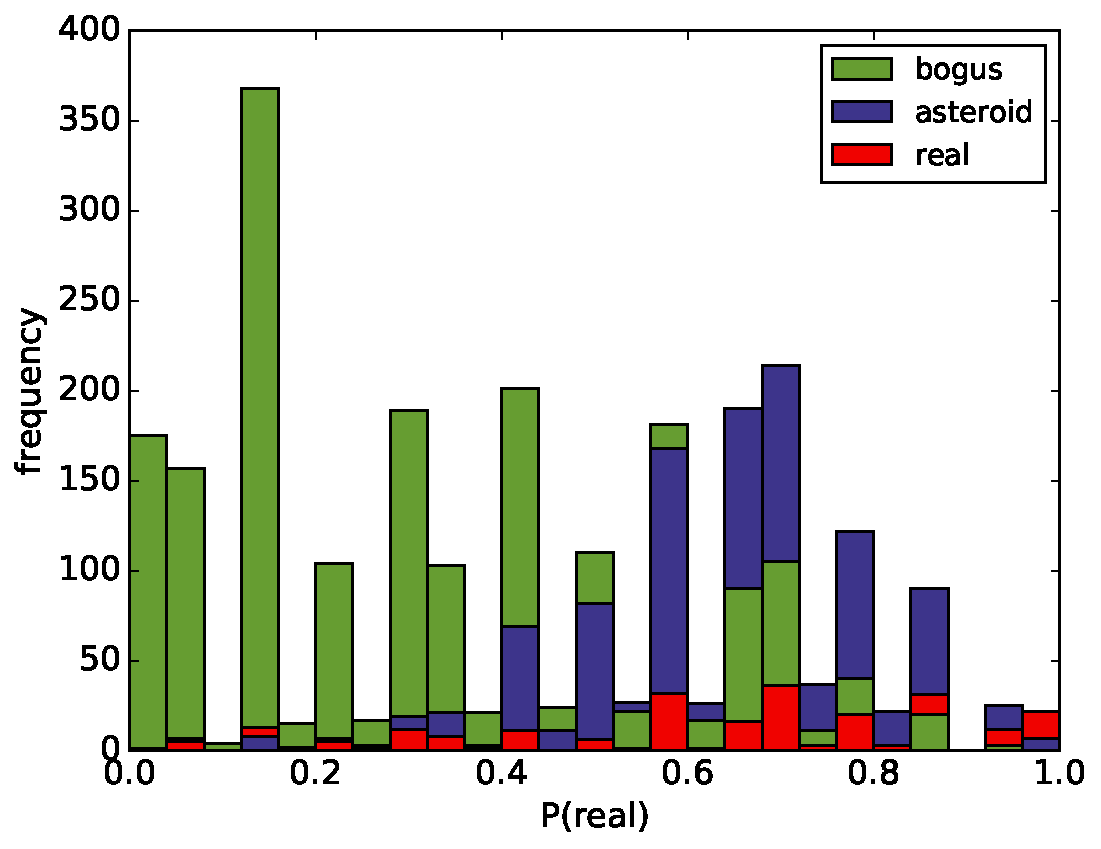
\includegraphics[width=84mm]{figs/human_hist.pdf}
   \caption{The distribution of $P(real)$ from Supernova Hunters for objects detected between 
            MJD 57570 and MJD 57586.  Compared with the machine $P(real)$ in ~\ref{fig:machine_dist}
            the objects at the extremes are pure.  There are very few real detections with 
            $P(real) < 0.04$ and few bogus detections above 0.92.} 
   \label{fig:human_dist} 
\end{figure}

Volunteer classifications were combined using the simplest possible metric; the fraction of volunteers who identified a potential transient is assumed to be an estimate of the probability of that candidate being real. Despite this simple procedure, the results show that volunteers could effectively distinguish between real and bogus classifications. However, the structure of the resulting distribution is strikingly different. Whereas for machine classification, a threshold could be chosen to give a complete but not pure sample, with volunteer classification it is easier to construct a pure sample of candidates which are highly likely to be supernovae, but this sample is far from complete. There are candidates judged `real' by experts even at low probabilities. 

Much work has been done in other projects to improve on this naive combination of volunteer votes. (XXXX Examples XXXX). However, such solutions have not yet shown to be generalisable between projects, and so require substantial effort in data analysis. They may also depend on large numbers of volunteers classifying each subject. Instead of pursuing this route, therefore, we combine human and machine classifications hoping to benefit from the different capabilities of both sets of classifiers. 

\subsection{Combining human and machines} 

Figure \ref{fig:combo_train} shows the combination of human and machine classifications. It is immediately apparent from the figure that no single threshold on either machine or human classification can outperform the combination of the two. This is an important result; it is the first time that the benefits of combining classification from both machines and volunteers has been clearly demonstrated using data from a real astronomical system. 

\begin{figure}
   %\vspace{200pt}
   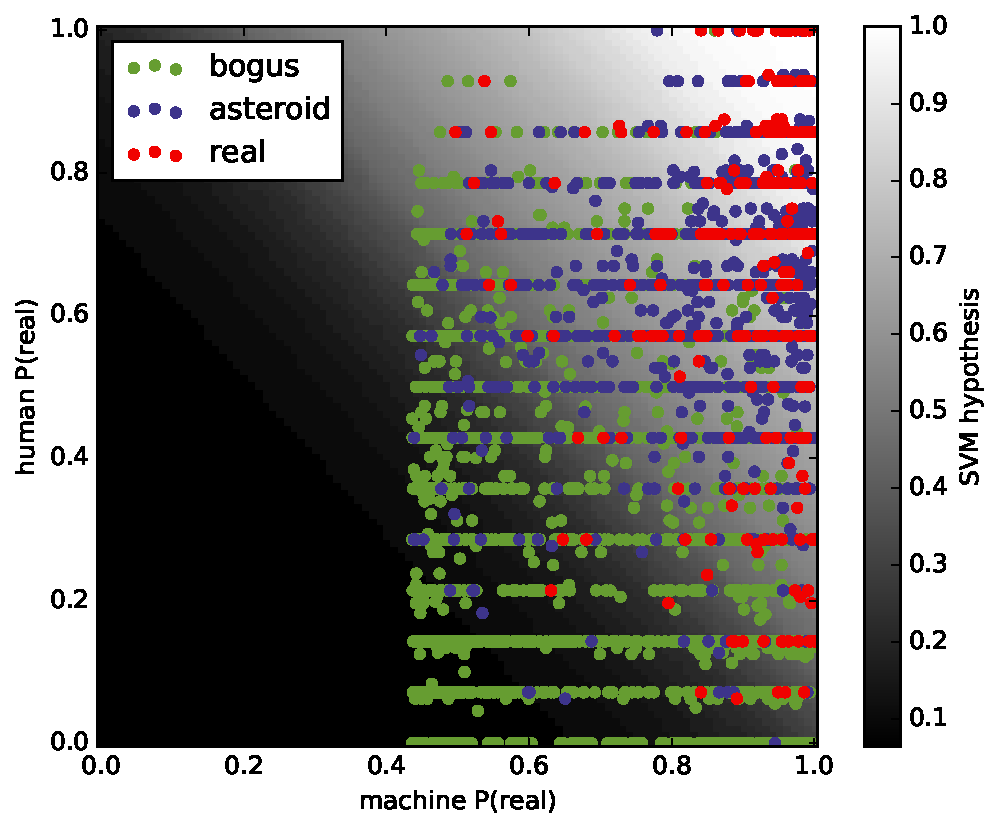
\includegraphics[width=84mm]{figs/human_v_machine_train.pdf}
   \caption{The $P(real)$ from Supernova Hunters against the machine $P(real)$ for detected 
            objects between MJD 57570 and MJD 57586.  Objects with machine $P(real) < 0.436$ are
            not uploaded to Supernova Hunters.  The background colour map shows 
            the $P(real)$ to that point in feature space by a linear SVM trained on the 
            examples shown. XXXX UPDATE GRAYSCALE XXXXX}
   \label{fig:combo_train} 
\end{figure}

How should the two independent classifications be combined? We use a linear support vector machine (SVM) with inputs consisting of both classifications, trained by the expert-labelled data. 

[XXXX put some equations XXXX]

The SVM  maximises the distance between populations of first `real' (and `asteroid') classifications and second `bogus' classifications, using only probability estimates from humans and machines as input. It was trained on the data discussed above, and the resulting score displayed as grayscale in figure \ref{fig:combo_train}. It was then tested on data processedsed between MJD 57587 and MJD 57607, with results shown in \ref{fig:combo:test}. This test shows that the combined classification performs well, and figures \ref{fig:roc} shows a comparison of the combined results for this test dataset with machine and human classifications on their own.


\begin{figure}
   %\vspace{200pt}
   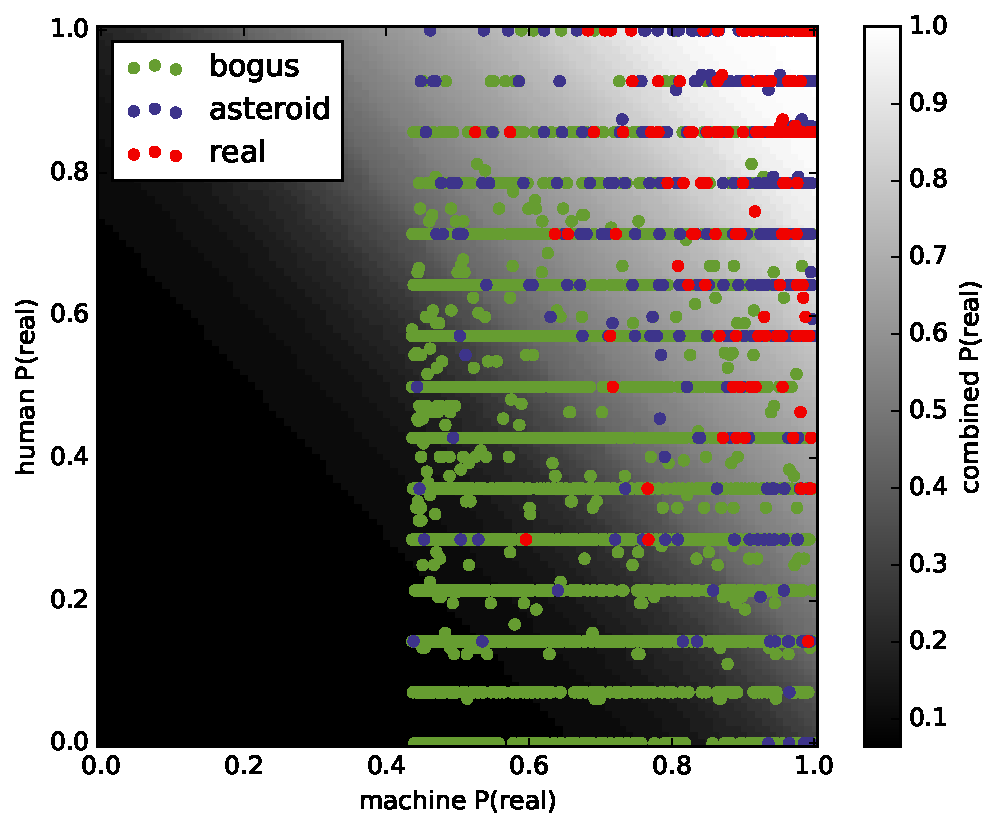
\includegraphics[width=84mm]{figs/human_v_machine_test.pdf}
   \caption{The same as ~\ref{fig:combo_train} but on a test sample of 4058 objects detected between
            MJD 57587 and MJD 57607 and held out during training of the linear SVM.} 
   \label{fig:combo_test} 
\end{figure}

\begin{figure}
   %\vspace{200pt}
   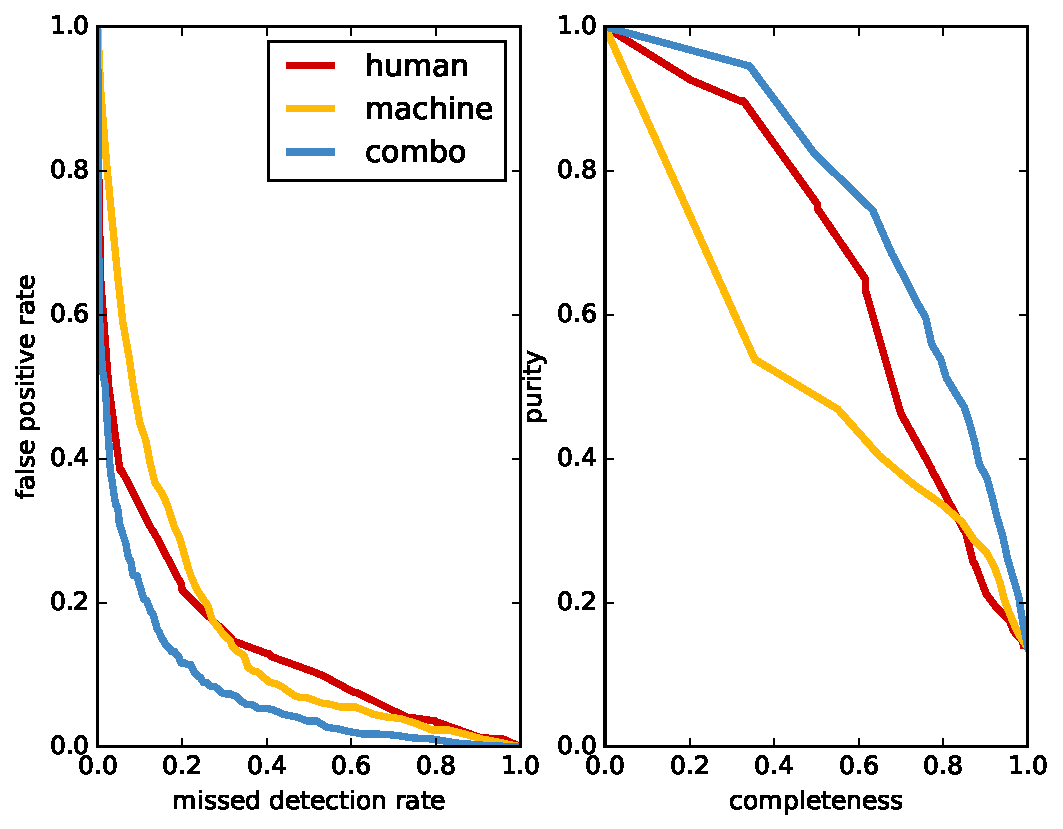
\includegraphics[width=84mm]{figs/roc.pdf}
   \caption{left: ROC curve showing performance measured on the test data in ~\ref{fig:combo_test} for human (red), machine (yellow) and
            the linear SVM combination of human and machine classifications (blue).  right: The equivalent Purity-Completeness curve.  Both
            plots show that the combination is always as good as or outperforms humans or the machine individually.} 
   \label{fig:roc} 
\end{figure}

\begin{table}
\begin{tabular}{|c|c|c|c|}
False Positive Rate & Human & Machine & Combination\\
1\% & 65.7\% & 91.1 \% & 55.1 \% \\
5\% & 49.4\% & 64.6 \% & 32.2 \% \\
10\% & 38.3\% & 44.9 \% & 22.7 \%\\
\end{tabular}
\caption{Missed detection rate recorded for a choice of false positive rates, based on expert classifications.}\label{tab:roc}
\end{table}

XXXXXXXX Calculate FPR for a variety of missed detection rates XXXXXX

\begin{table}
\begin{tabular}{|c|c|c|c|}
Missed Detection Rate & Human & Machine & Combination\\
1\% & 100\% & 94.3\% & 84.9\% \\
5\% & 73.0\% & 65.4\% & 42.4\% \\
10\% & 60.8\% & 39.2\% & 23.7\%\\
\end{tabular}
\caption{False positive rate recorded for a choice of missed detection rates, based on expert classifications.}\label{tab:roc}
\end{table}

For any choice of false positive rate, the combination of classifications produced a lower missed detection rate. Equally, for any required purity or completeness the combination produced a better dataset. 

\section{Conclusions}

\textbf{CJL}

\bsp	% typesetting comment
\label{lastpage}
\end{document}